\documentclass[12pt]{article}
\usepackage{navigator}
\usepackage{mathtools} 
\usepackage{graphicx}
\usepackage{subcaption}
\usepackage[a4paper, total={6in, 9.5in}]{geometry}
\usepackage{float}
\usepackage{url}
\usepackage[margin=.5in, labelfont = bf]{caption}
\usepackage[normalem]{ulem}
\usepackage{xcolor,cancel}
\usepackage{setspace}
\usepackage{blindtext}
\usepackage{multicol}


\linespread{1.15}
\graphicspath{ {./images/} }

\begin{document}
    \title{Widget Lab 3}
        \author{Robert Purcaru [1007019842]}
        \date{\today}
    \maketitle

    \includegraphics[width=\linewidth]{White.png}
    \includegraphics[width=\linewidth]{CN.png}

    % \begin{figure}[H]
    %     \centering\includegraphics[width=0.7\linewidth]{StepperWiring.PNG}
    %     \captionsetup{width=0.9\linewidth}
    %     \caption{Stepper Wiring Taken From Lab Manual \cite{LabManual}.}
    % \end{figure}

    \newpage

    \section*{Executive Summary}
        Many developing countries are hindered by a lack of waste management infrastructure, especially when it comes to sorting and recycling plastics. Recycling centers are few and far in between, leaving many people to dispose of their waste in landfills, mixing recyclable and non-recyclable materials together. In recent decades, several projects have sprung up to address this growing crisis \cite{wansi_2022} \cite{dow_2022}. Still, much of the plastic waste sorting is done by hand by individuals sorting through landfills for recyclable plastics \cite{GhanaSorting}.

        Given the nature of the context, our team developed a value proposition to help us align our work with a greater, overarching goal that could help guide our design to something that could tangibly help our stakeholders. We set out to design, develop, and demonstrate an aid for the plastic waste crisis that does not require attention at the point of waste introduction, that reduces the burden on existing infrastructure, that increases recycling throughput, and that does so while maintaining or creating relevant jobs.

        Through our research, we identified several ways of sorting plastics, however settled on a combination of density and colour as they seemed to provide relatively clear distinctions \cite{gent2009recycling} \cite{safavi2010sorting} \cite{bruno2000automated} with the most feasible implementation. Given the necessity to operate under constraints set by our FaCTs, our final prototype was scoped to demonstrate the concept of a density and colour based sorting system made with easily available mechanical and electronic materials\footnote{Namely, those available at MyFab.}. If such a system could work, we would successfully have shown that there is enough information in just the colour and density of a plastic to devise a practical sorting system that could separate recyclable materials, broadly, from non-recyclable ones. Being a system that requires some human supervision and assistance, this kind of design would address every aspect of our value proposition. 

        Our final prototype consists of 2 main features: an optical, traversing scanner and a rotating, weighing plate. The scanner was initially intended to be a camera that would traverse over the subject material, however this was scoped out early in the design process, leaving our group to instead develop our own optical scanning assembly. Through a combination of red, green, and blue LEDs, our design shines different lights on the subject material and observes the reflected light using photoresistors. By traversing over the subject, we can generate an image profile under different lighting conditions and, in combination with the weight information form the scale, determine an approximate density of the plastic. Then, by comparing the result to reference data, the platform tilts in one of two direction, sorting the material into one pile or another.

    \newpage

    \tableofcontents

    \newpage
\begin{multicols*}{2}
    

    \section{Introduction}
        \subsection{Value Statement}\label{subsec:ValueStatement}

            Many developing countries are hindered by a lack of waste management infrastructure, especially when it comes to sorting and recycling plastics. Recycling centers are few and far in between, leaving many people to dispose of their waste in landfills, mixing recyclable and non-recyclable materials together. In recent decades, several projects have sprung up to address this growing crisis \cite{wansi_2022} \cite{dow_2022}. Still, much of the plastic waste sorting is done by hand by individuals sorting through landfills for recyclable plastics \cite{GhanaSorting}.
            
            Four significant facts have been identified by our Global Context Provider (GCP): 

            \begin{enumerate}
                \item Sorting at the point of waste introduction is uncommon; people don't tend to sort their trash from recyclables.
                \item Recycling locations are few and far in between.
                \item People recognize the value in sorting their plastics, both environmentally and economically. 
                \item People recognize that a better solution for plastic sorting is necessary.
            \end{enumerate}

            Our GCP further stressed the importance for the need to focus on sorting at the point of collection, reducing the burden on waste pickers to increase recycling throughput.

            Important in developing a product that truly helps a community is addressing the sustainable development of that community. The United Nations Sustainable Development Goals (UNSDGs) \cite{UNSDG} provides 17 goals to achieve in developing countries to produce a sustainable future. This opportunity provides the chance to address Goal 1: No Poverty by developing jobs in waste management, Goal 9: Industry, Innovation, and Infrastructure by instantiating infrastructure to set the precedent for future development, Goal 11: Sustainable Cities and Communities by retrofitting existing public works for sustainable waste management, and Goal 14: Life Below Water by reducing the impact plastics and landfills have on bodies of water.

            The combination of these factors leads us to our team's value statement:

            \textbf{To design, develop, and demonstrate an aid for the plastic waste crisis that does not require attention at the point of waste introduction, that reduces the burden on existing infrastructure, that increases recycling throughput, and that does so while maintaining or creating relevant jobs.}

        \subsection{Our Design}
            We devised and developed a plastic sorting machine that would sort materials into two groups by measuring their density and colour, thereby reducing the load on waste pickers. Through our research, we identified several ways of sorting plastics, however settled on a combination of density and colour as they seemed to provide the clearest distinctions \cite{gent2009recycling} \cite{safavi2010sorting} \cite{bruno2000automated} with the most feasible implementation. 
            
            Our design consists of two cooperative systems: a pivoting scale, and an optical scanner. By  measuring the volume and color composition of a given set of materials, our design seeks to separate various materials based upon this distinction. The machine can be set to separate a variety of different materials, performing a binary search like process if run multiple times.

            Our design can be implemented at the point of collection to reduce the burden on plastic pickers by sorting batches of materials into piles that are more and less likely to be recyclable. This could increase the throughput of recyclable material by decreasing the time it takes to separate recyclable materials from non-recyclables while still requiring a worker to introduce material to the sorter and perform a final, more refined sorting of the desired pile.

            
            \begin{figure}[H]
                \centering\includegraphics[width=\linewidth]{InitialConcept.png}
                \captionsetup{width=\linewidth}
                \caption{Initial sketch of our design idea. Design is exploded in x-direction for clarity. Initial design incorporated flattening machine which was scoped out early in design process.}
                \label{fig:initial}
            \end{figure}

    \section{Background}
        \subsection{Stakeholders}
            First and foremost among our stakeholders is the GCP, Adwoa Coleman. Being the only person we had the opportunity with on-the-ground experience in the environment in question, our design is built to address her specifications; the situation she presents is the one we're designing for.
            
            Equally impacted by but less accessible to us are the people living in Ghana whom our solution may affect either directly affect (i.e. garbage collectors, recycling workers, etc.) or indirectly affect (i.e. people in Ghana producing and feeling the impact of pollution). This group of stakeholders is the most broad as it houses everybody besides Adwoa Coleman that may be impacted by our design but whose personal experience remains allusive to us. Still, they are largely the focus for the impact of our design.
            
            Finally, the last group of stakeholders we consider are all the people involved with the ESC204 course, including but not limited to: our team, the FaCTs, MyFab and other ESC204 teams. This group of people will likely feel the most direct affect of our work while influencing the design decisions we make. It is worth noting that this group of stakeholders serves as a practical grounding for our design; the scope of the implementation of our design is necessarily limited by the overarching scope of the ESC204 course. 

        \subsection{Scope}
            Our design seeks to improve upon a job that is already performed relatively quickly by human workers. Such an ambitious goal requires thorough justification and testing before final development and implementation. Accordingly, our primary goal was to test the feasibility of a color and density sorting system made with relatively low cost materials. An ultimate implementation of our design would seek to address select UNSDGs as outlined in section \ref{subsec:ValueStatement}, doing so if and only if our testing and attempts at optimization demonstrated that our design could indeed improve sorting throughput.

            The scale and degree to which we could test our concept was limited by the materials available to us and the time we had available. Our original design concept called for a camera to act as a sensor, however supply limitations excluded this from our scope, leading our team to develop our own light and color sensor. The scope of our solution can be observed to change as the design constraints were adjusted by the FaCTs stakeholders. Ultimately, the limitation to scope imposed by materials was limited to that which could be acquired in reasonable quantity from MyFab based upon their stock at the time. 

        \subsection{Environment}
            Ultimately, our design would be expected to work alongside waste pickers to ease their burden of sorting. It should therefore be portable, rechargeable, and rugged enough to withstand regular use and abuse. Ghana also experiences dry and wet seasons; the solution should be able to function in heat exceeding 40$^o$C \cite{GMET}. Any enclosure designed for our product would be expected to do all this while presenting a safe and easy to maintain form factor so as to allow for on site, or otherwise, simple maintenance. 

        \subsection{Prior Designs}

        \subsection{Requirements}
            At a high level, our solution is expected to improve the throughput of plastics from landfills to recycling facilities. The design should accomplish this by analyzing a sample to gather information about density and color. Then, it should determine if it is likely to be recyclable by comparing the analysis to a reference dataset before dispensing it onto one of two piles. 

            For the purposes of proving the concept that sorting plastics based upon density and color is sufficient to distinguish between recyclable and non-recyclable samples, the design must be able to successfully sort individual samples of both recyclable and non-recyclable materials, with no further constraints. This proof of concept would act as the basis for either further development into a final product or dismissal of the concept, making this requirement critical above all others. Assessment of this requirement would be carried out by comparing the sorting the final product could achieve compared to what a perfectly sorted set would look like. That is, each piece of unsuccessfully sorted plastic would be a point against the concept. There is no use in setting an exact bar as to what would be acceptable as a human would be required by the value proposition for post-process handling and curating of the material, however by producing a piles which are sorted to a greater degree would be preferable.  

            With the concept proved, the performance of the ultimate design should be tested by introducing a variety of materials (recyclable, non-recyclable, as well as a combination of the two) to ensure that a great proportion is sorted correctly to minimize subsequent screening time of the sorted pile. The design should also be tested against a human subject to determine if any improvement is achieved against human performance. Doing so would involve the human feeding material into the machine as quickly as it could handle it and assessing its performance there. In this respect, the design would be considered acceptable if it meets or outperforms the individual, as either of these would represent an improvement upon the current circumstances. This requirement would only need to be met by a final design, not necessarily the prototype produced to demonstrate the concept. 

            For the enclosure, to achieve the desired waterproofing, IPX4 \cite{gniazdo_2021} or greater should be met and demonstrated against the standard IPX testing procedures. To address heat in the environment, no materials should be used that warp or become damaged in temperatures approaching 50$^o$C \cite{GMET}. This could be verified using a space heater, a thermometer and a small enclosure to leave the design exposed to. 

    \section{Design Process}

        \subsection{Overarching \\ Design Decisions}
            Key among our design decisions was to use an combination optical, density sensing machine to determine if a sample could be recycled. Through our research, we were unable to find a product or design that incorporated these as a distinguishing mechanism on the scale we were targeting. Our research did however show that while recyclable and non-recyclable plastics have similar densities \cite{omnexus_2021}, the applications of recyclable plastics like PET, HDPE, and PE tend to be used in products like bottles, containers and bags \cite{HDPE} \cite{amp} \cite{omnexus_2017}, which can have a lower apparent density, given their enclosed air content\footnote{This is partly due to the manufacturing techniques these plastics lend themselves to \cite{thomas_2022}.} and tend to be partially transparent to some or all colours. Our decision to use density and colour as a basis for sorting was therefore informed by our research into the properties of recycled plastics. 
            
            Our decision to make a product which could be used by waste pickers on site was informed by our value statement; we wanted to develop something that could work unsupervised and ease the burden on waste pickers to increase the throughput of recyclable plastics. Plastics are generally identified by a small number molded into the item \cite{plasticactioncenter_2022} for human interpretation. Our design sought to remove the requirement that a human check every piece of potentially recyclable plastic for its identifier by reducing the size of the pool of plastics they were checking. By providing a human sorter with a partially sorted pile of waste, the volume of recyclable material the human can process should increase.  

        \subsection{Prototyping and \\ Application Design \\ Decisions}
            Fundamentally, our design sought to determine the practicality of a density and colour based sorting solution. To this end, our team planned to do much of our testing and work in software by using a camera as the basis for most of our measurements. Unfortunately, as the scope of our design shifted, narrowing the availability of materials, our group had to refocus our attention on how spatial and color information could be determined without a camera.

            Our first round of testing was to determine if the photoresistors available at MyFab would be sensitive enough to act as our main optical sensors for either colour or simply area and volume. Cadmium sulphide photoresistors are sensitive to the vast majority of the visible light spectrum, but slightly more so to blue light than any other \cite{eepower_2017}. Knowing this, we tested the sensitivity with 5 different materials of varying darkness and opacity and found that resistance varied enough to distinguish between the materials. To test whether or not the photoresistors would be sensitive enough to colour to act as color sensors, we illuminated samples with coloured LEDs and found that when the colour of the LED was close to the color of the material, the resistance also changed measurably between trials. Most importantly however, in all the trials, the resistance was stable to about 1 part in 1000. This meant that the photoresistors would be sensitive enough to use as optical sensors in our final design.
            
            In order to transduce the varying resistance of the photoresistor to an analog signal our microcontroller could interpret, we started with a voltage divider. However, this limited the operational range of the signal, since the photoresistor's resistance varied between about 4k$\Omega$ and 8k$\Omega$ before going to an open circuit. To address this, our team tested a non-inverting amplifier circuit using an operational amplifier (opamp) to allow the signal to vary between 0V and the V$_{cc}$ of the microcontroller. 
            
            \begin{figure}[H]
                \centering\includegraphics[width=0.7\linewidth]{OpAmpSch.PNG}
                \captionsetup{width=\linewidth}
                \caption{Schematic representation of non-inverting amplifier circuit used with photoresistors.}
                \label{fig:opamp}
            \end{figure}

            The benefits of this were threefold: first, our sensors operational range increased to encompass the full range of ADC values, increasing our measurement resolution. Second, it does so while protecting the microcontroller from overvoltage as the rail-to-rail opamps we used saturate at the supply voltages. Third, the supply for the photoresistor voltage divider could be a 5V LDO, meaning the supply noise would be filtered and minimized\footnote{This is opposed to using the 12V switch supply used to drive the motors, which had considerable noise.}. After adding sets of red, green, blue, and yellow LEDs, our color sensing concept had been demonstrated, allowing us to move on to the platform that would carry it. 

            Our first scanning prototype involved an array of 8 photoresistors on a 1/4" birch dowel rail system pulled by a stepper motor. While this did demonstrate that our design could scan a surface with some accuracy, the resolution and rail system were ultimately inadequate. To address the former, we added another 7 photoresistors and removed the yellow LEDs since the yellow results were indistinguishable from having red, green, and blue all on together. We also found that running the LEDs with microcontroller power supply was inadequate as the current it could supply was too low for the required brightness. To address this, we used a series of MOSFETs to act as low-side switches for the LEDs, powering them with the same power supply that was running the motors.
            
            To address the rail system, we redesigned our pulling mechanism to be driven by a threaded rod rotating inside a captive nuts on our sensor gantry, allowing it to be moved in both directions on its axis. Both of these changes dramatically improved the performance of our design for both speed and resolution.

            \begin{figure}[H]
                \centering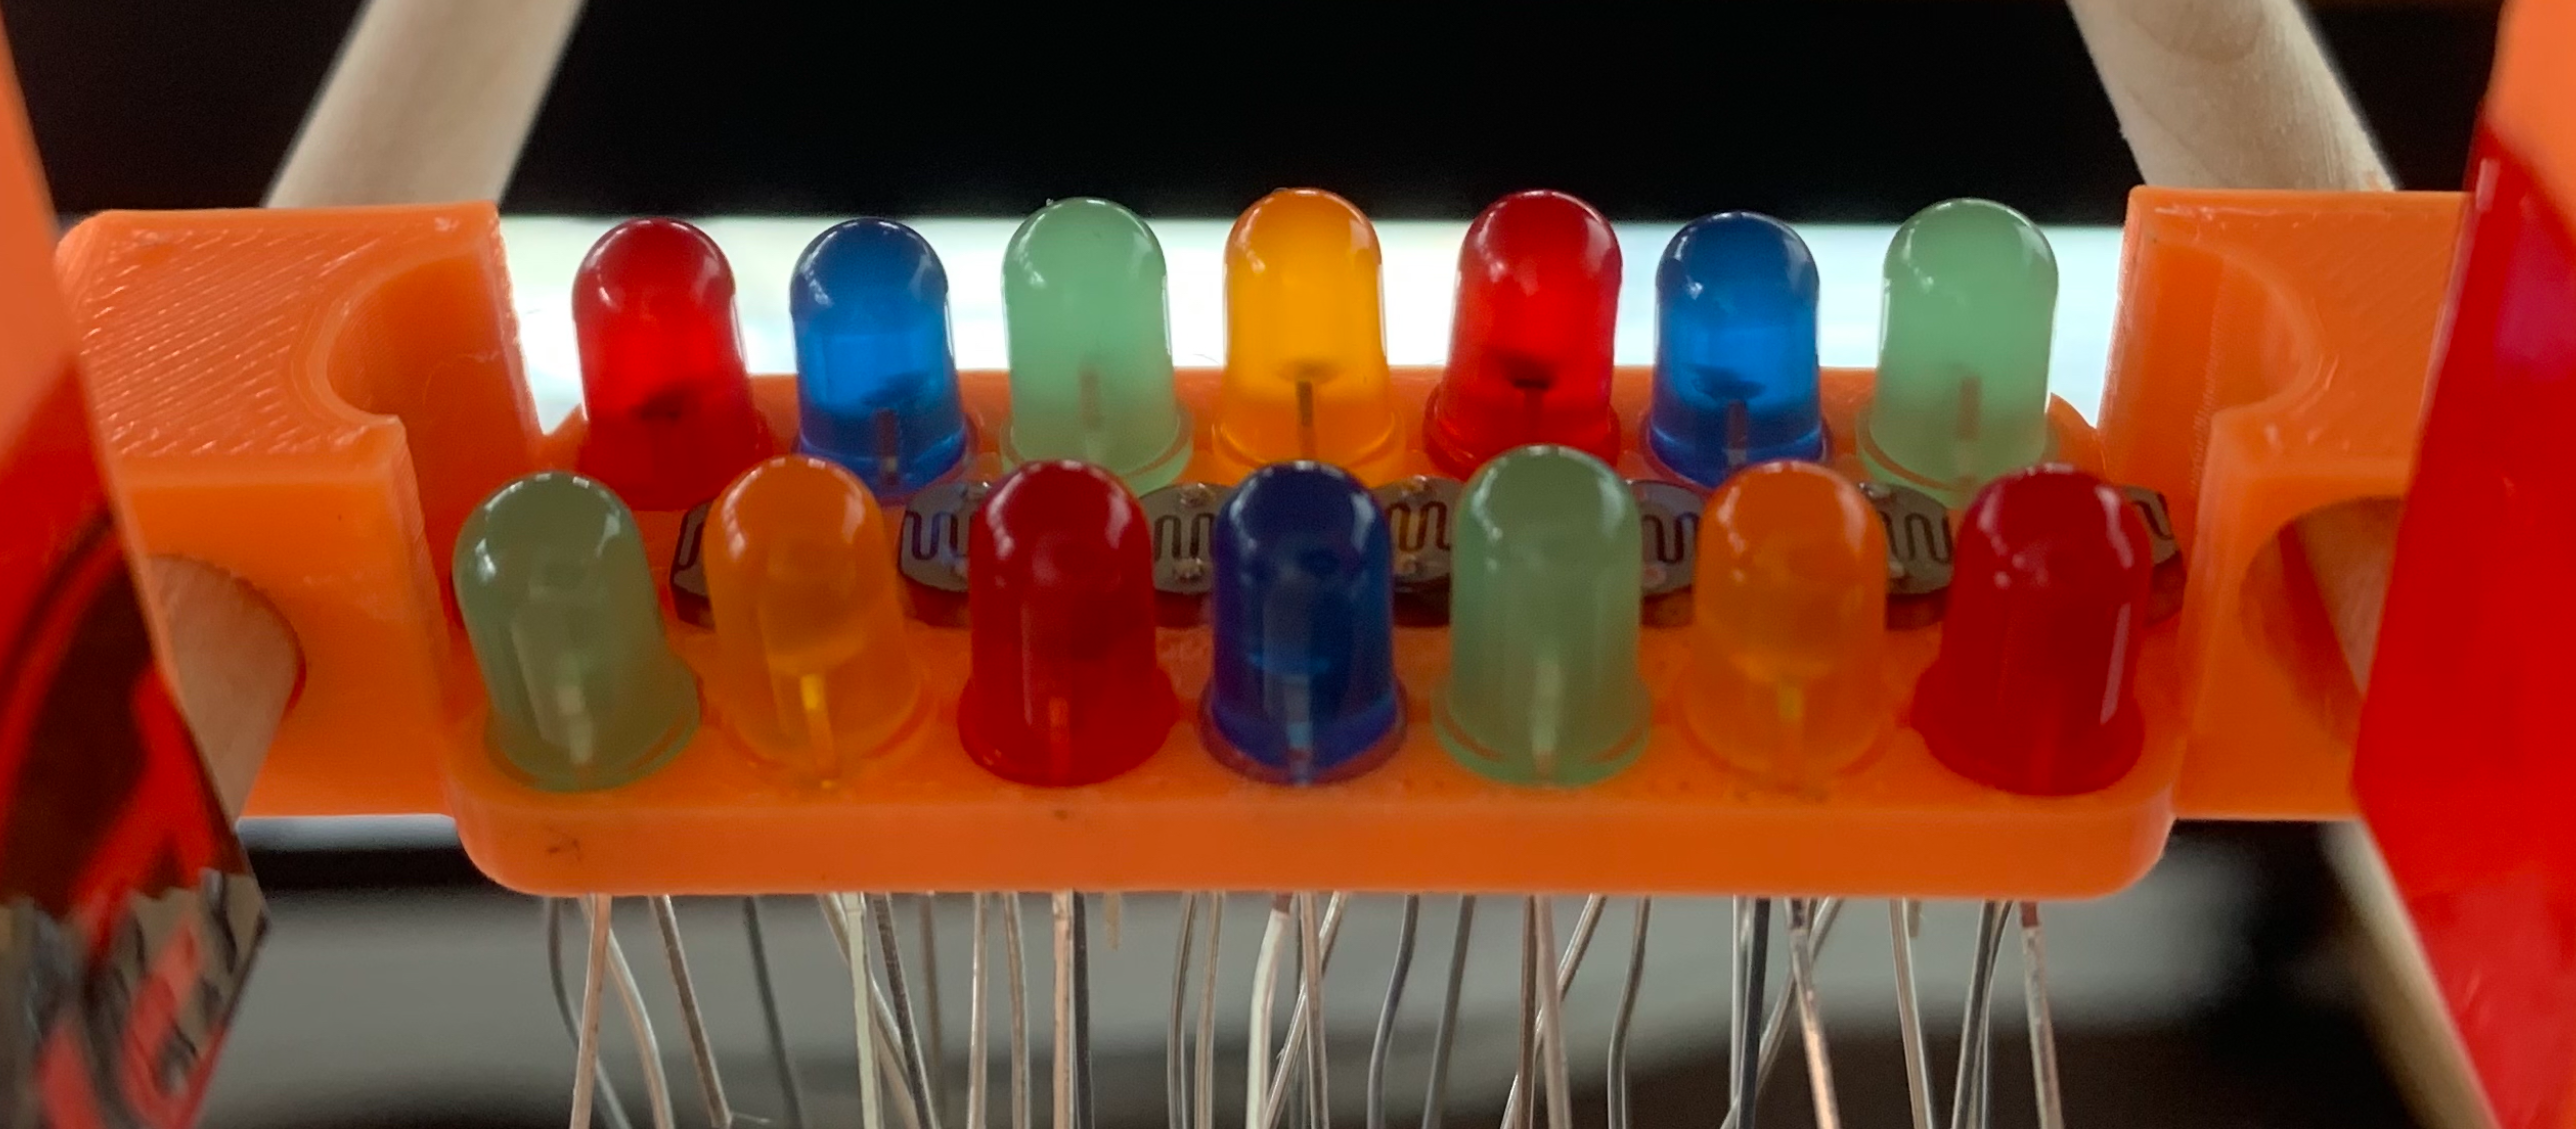
\includegraphics[width=\linewidth]{LEDs.PNG}
                \captionsetup{width=\linewidth}
                \caption{Photoresistor and LED arrays on first scanning prototype.}
                \label{fig:LEDs}
            \end{figure}

            \begin{figure}[H]
                \centering\includegraphics[width=\linewidth]{ScannerV2.png}
                \captionsetup{width=\linewidth}
                \caption{Photoresistor and LED arrays on final prototype. More photoresistors were added and the yellow LEDs were removed. Density of each was also reduced after testing first prototype.}
                \label{fig:LED0sV2}
            \end{figure}

            \begin{figure}[H]
                \centering\includegraphics[width=\linewidth]{BirdsEye.PNG}
                \captionsetup{width=\linewidth}
                \caption{Overhead view of first scanning prototype. Original rail system had a stepper motor pulling gantry with wire.}
                \label{fig:Overhead}
            \end{figure}

            \begin{figure}[H]
                \centering\includegraphics[width=\linewidth]{CarriageV2.png}
                \captionsetup{width=\linewidth}
                \caption{Overhead view of final scanning prototype. Final rail system is driven by a threaded rod driving captive nuts in the carriage. Wooden dowels on either side keep assembly aligned.}
                \label{fig:OverheadV2}
            \end{figure}

            The scale and rotator, being the simplest and most \textit{believable} part of our design was prototyped in a limited fashion. Testing of the load cell was done quite late in the design process, however it provided the desired resolution without much work. The rest of the platform was designed and manufactured late in the design process but also worked as intended without problem.

        \subsection{Project Management}
            
        \subsection{Reflection on Global Virtual Interaction}
            Unfortunately, our team was unable to gather much useful input from our GSU partner through our interactions or their feedback. While the GSU student had some interesting insight on the context and their interpretation of the opportunity, we were unable to divine much in the way of useful or guiding information from the interaction, despite our good-faith attempt to have them elaborate on their feedback to elucidate their ideas. 

            It seemed that our GSU collaborator was suggesting ways in which we could better understand what exactly it was about the process of material collecting and sorting that was so arduous as to warrant a helping design, however this was addressed in the context provider's statement. Our understanding lead us to believe that the groups that tend to take this kind of work are among society's most vulnerable, potentially leading to exploitation. Additionally, the work itself can be taxing as it involves sorting through potentially hazardous materials for many hours throughout the day. Despite explaining that our design would seek to address this by reducing the worker's direct exposure to the hazardous materials by partially sorting waste, our partner never elaborated on their point. 
            
    \section{Final Design}

        \subsection{About the Design}
            Our final design carried some aspects from our prototypes forward while addressing many of the greater pitfalls in the original design. First, one of the greatest problems with the design was the wiring. Constraints presented to us by the FaCTs effectively scoped out using anything but jumper wires everywhere as they could be disassembled easily. Our team pushed back against this constraint for our final design, owing to the undue difficulty and limitation this forced upon us; a rugged solution would be impossible to achieve without proper harnessing between the gantry and the rest of the system. As a result, our team moved to soldering the components on the gantry to prototyping boards and wiring those to the breadboards our microcontroller and ICs were mounted to. This reduced the impact the harnessing had on our design, allowing for a more rugged design to meet our requirements. 

            Our final design also addressed motion of the gantry, which was lackluster in our prototype. By using a threaded rod to drive a pair of captive nuts, we not only increased the rigidity of our system, but also increased the resolution in the axis of the rod by having much more precise control of the position of the gantry. This helped us achieve our requirement of accurate and consistent sorting materials by color and density through the improvement in resolution and repeatability.

            Our initial design solution to sort waste and recyclables was a paddle that would swipe left or right across the platform to push the material to either side. For our final design, we made the entire platform tilt left or right, driven by a motor through a gear stage. This design is more robust and representative of how the solution might actually be implemented in context. For instance, the paddle needs to be positioned such that it faces away from the platform so that it can access the entire surface; in this way, the whole design must be twice as long as the platform itself. In contrast, if the platform simply tilts to drop material to the designated side, the design remains compact. This becomes especially useful when considering a larger sized implementation of the solution.

            \begin{figure}[H]
                \centering\includegraphics[width=\linewidth]{WholeDesignGrass.png}
                \captionsetup{width=\linewidth}
                \caption{Whole design assembled together. Pivoting scale platform can be seen underneath scanning deck. Sensors and LEDs are all wired in the main harness connected to the scanner (cluster of wires right of center.) Breadboard nearest to viewer holds opamps and signal transduction circuitry. Leftmost breadboard holds servo drivers and power regulators. Breadboard farthest from viewer holds LED control MOSFETs.}
            \end{figure}

        
            

        \subsection{Performance, \\Limitations, \\and Justification} \label{subsec:PerformanceLimitationsJustification}

            Through the final testing our group conducted, we were able to achieve some of the performance we sought for; our first and final prototypes indicate that a solution with colour and density sorting is feasible within the context provided. Our final design is able to identify and sort materials like plastic bags, bottles, containers, and loose scraps from heavier, non plastic materials. It is able to successfully identify and record the shape of the scanning subject while weighing it and collecting color information. 
            
            \begin{figure}[H]
                \centering\includegraphics[width=0.5\linewidth]{ScannedImage.png}
                \captionsetup{width=\linewidth}
                \caption{Image observed by scanner of opaque, empty plastic pouch. Made by exporting 2D array generated with scanner and visualized with OpenCV library.}
                \label{fig:ScannedImage}
            \end{figure}

            It is however less successful when it comes to distinguishing between recyclable and non-recyclable plastics. The resolution of the density is not fine enough to do so in some cases and in others the plastics are simply too similar to distinguish. Still, this falls within our requirements; the partially sorted pile the design produces requires some human attention, but is still more sorted than the originally introduced pile. 

            The major pitfall of our design is the speed with which it scans. The design is limited by two factors: first, the microcontroller we used - ATMEGA 2560 - takes an appreciable amount of time to read, store and offload all of the analog signals from each of the photoresistors and advance the stepper motor. This is generally because of the abysmal ADC performance on Arduinos and the relatively slow clock speed (16MHz) the microcontroller runs at. And second, the LEDs have a significant (tens of milliseconds) time to turn on to full brightness once they are enabled. This has to do with the switching characteristics of the IRF510 power MOSFETs as well as the 5mm LEDs available to us through MyFab. Both of these limitations to speed can be addressed in future iterations (see section \ref{subsec:NextSteps}) but do not detract from the potential efficacy of the design, they only arise as a result of course-material limitations. Still, it seems like speed would likely be a major limitation any small scale implementation of this design. A human, while not very quick, can still be very competitive with our design, calling into question the validity of this kind of implementation of a colour and density sorting solution\footnote{This is not to say that colour and density sorting is not feasible, only that the scope our team operated under may not have left room for a valid solution.}.   

            There are also several aspects of our requirements we weren't able to test completely. For example, one of our requirements states a worker must be able to use this with them outside of a recycling facility. While our team did calculations to determine that 8 AA alkaline batteries in series could supply our design with the requisite current and voltage, we were unable to assemble a battery pack to test this with; we only tested with a power supply and regulator for the microcontroller. Technical limitations like these can be broadly be addressed (see section \ref{subsec:NextSteps}) but tend to push the scope of the project and design.           
            
            In summary, we achieved the spirit of our value statement. With more time, we could feasibly implement a design that explicitly achieves every aspect of the statement with a broadened scope for materials and time. Our testing and design demonstrated an ability to sort plastic at the point of introduction, reducing the load on workers\footnote{Albeit in a limited capacity.}, allowing for increased throughput of plastics through the recycling system without eliminating jobs.  


        \subsection{On Our Team's Interaction}
            Our team chose not to follow a strict division of labor for the development of any of our prototypes, everybody helped wherever they could whenever they themselves were not leading some aspect of the design. A key example of this is with the wiring in our first prototype, shown in figure \ref{fig:Overhead}. The wiring was incredibly tedious and needed to be perfect. It would have taken one person alone a few hours to do it properly and test it, however by splitting up the work and not assigning one person alone to it, we were able to finish the prototype faster than we otherwise would have. 

            Of course, there were areas where one team member was more experienced than the others and was left to lead the corresponding part of the process. In these situations, the person would try to help the others understand what they were doing and why, however not at the cost of productivity. As is discussed in our Team values Statement (see Appendix \ref{subsubsec:TVS}), our team valued work well done over immediate understanding of a concept. This allowed our team to not get bogged down in explanations during the prototyping process while ensuring everyone understood what was going on by sharing an understanding after the fact.

    \section{Conclusion}
        \subsection{Reflection on Final Design}
            In principal, we achieved the first part of the potential implementation of this product; we demonstrated that color and density can act as a basis for sorting some recyclable materials before human intervention. In doing so, we realized the value statement, while appropriate for the context, set the scope too deep for the time and resources we had available. While we were able to get through two partial design cycles - reframing and reassessing our requirements and scope - we were unable to produce a final product which could be used in the context we were addressing with our value statement. Still the insight we gained allows us to reflect upon our initial value statement and reinforce it. It seems that the concept of a compact, onsite, density and colour based sorter has the potential for in-context implementation, but requires further development before such an implementation can be achieved. This is supported by the functionality our final prototype affords, proving that it is possible to achieve some degree of sorting with the technology, despite the limitations discussed in section \ref{subsec:PerformanceLimitationsJustification}.

        \subsection{Next Steps} \label{subsec:NextSteps}
            Future iterations of this design need to address 2 major aspects of value statement.
            
            First, to increase throughput, the machine must work with a worker to outperform the worker doing the same task on their own. This would involve speeding up the sorting process and overcoming some of the limitations of the design, as discussed in section \ref{subsec:PerformanceLimitationsJustification}. To this end, our team suggests three major changes. First, switch to a 2-core STM based control system to operate at higher speed and take full advantage of multithreading to increase scanning performance. This would require the addition of an analog multiplexer to maintain the resolution achieved by our prototype without requiring the microcontroller to have as many internal ADCs, saving on cost. Second the power MOSFETs should be replaced with ones that have a lower gate charge and quicker I$_D$ response to V$_{GS}$, allowing the switching time for the LEDs to decrease and the duty cycle of a single scan to be decreased. Finally, a small, cheap camera should be used to replace the photoresistor array and eliminate the scanning motion required, instead relying on the microcontroller to process the image reported by the camera. Parts of the design would be kept (LEDs, scale platform), but the main gantry on the top would likely be removed in exchange for a camera\footnote{Testing contingent.}. Additionally, the addition of a second axis should be seriously considered to increase the significance of the density measurement. Doing so would allow us to form a quasi-3D image of the subject, making the density measurement more significant and aiding with sorting reliability.
            
            Second, once it is confirmed that the concept can provide value to the context, a great deal of work needs to be done on the packaging side of the design to bring it within specifications of the requirements. Unfortunately, the time we had did not permit us to develop an enclosure suitable for the context. It wouldn't have made sense to design an enclosure without knowing if the design could work, however we did investigate sealing techniques and temperature ratings for all the components we ended up using; nothing in the existing design should degrade considerably at higher temperatures\footnote{According to available datasheets and specifications.} but some parts can certainly become damaged by excessive exposure to water or moisture, leading to corrosion. This would need to be addressed in a final iteration. 

    \newpage

    \bibliography{References.bib}
    \bibliographystyle{ieeetr}

    \newpage

    \section{Appendix}
        \subsection{Team}
            \subsubsection{Team Values Statement} \label{subsubsec:TVS}
            As a team, we prioritize safe, durable and sustainable solutions. Prior to the development of our conceptual design, we knew that we wanted to ensure all possible value of plastics could be obtained through a sustainable, effective, and safe preliminary waste sorting process. We did not want to be a team that would provide a solution, that, while innovative and pleasing to the eye, would not provide value outside of this course. 
            Through our research on the community of Ghana and their waste management infrastructure, we realized that prioritizing a sustainable and durable solution would be able to prevent further harm to the community in ways that were not mentioned in their opportunity statement. We had discovered that most of the waste pickers make about GHS 2-5 per day and are elderly women, the most vulnerable members of any society. As such, we aimed for a safe and socially sustainable solution that was not 100\% automated to maintain jobs. 
            The street pickers, while they receive a daily salary less than minimum wage, earn significantly less during the rainy season. The rainy season brings flooding which prevents collection and washes away usable material. As such, we were aiming for a durable solution to address the fact that the solution is going to be implemented in extremely wet, unsanitary, and difficult working conditions.

            \subsubsection{Benedek}

            \subsubsection{Charles}

            \subsubsection{Katarina}

            \subsubsection{Robert}
                The majority of my prior experience in design has been with electronics and some mechanical design. I took it upon myself to lead, wherever I could, in the electronics portions of our designs and work out the finer details of how the more complex components, like how the opamps and MOSFET control would work.

                I value practicality and attainability in my design work; my contribution to the values statement was to assure that anything we set out to design was within our capabilities and attainable within the scope of the assignment. Additionally, I see value in thoroughly developing one part of a design and confirming its efficacy before moving on to another. This was borne out not only in our value statement but the scope of our final prototype; it is more valuable to rigorously test the concept of colour and density sorting than it is to design a product assuming that and have it fail in the end. 

                For our project management, I organized and coordinated all aspects of the design with my teammates. I made sure that each separate part of the design could integrate with the others and produce a final prototype which performed as we wanted it to. This was important to my values as, again, having several pieces which worked independently but not together would produce a prototype that would ultimately fail. 

                Therefore, my motivation, goals, and organization strategy helped with our team's success by keeping us grounded and allowing us to make deliberate and effective design decisions while scoping and executing our design.


            \subsubsection{Ria}

            
        \subsection{Bill of Materials}


\end{multicols*}

\end{document}